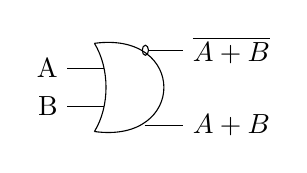
\begin{tikzpicture}[x=.49cm,y=.8cm,font=\sitneoznake]
\draw(0,0)..controls(.4,.4)and(.4,1)..(0,1.4);\draw(0,1.4)..controls(1.2,1.5)and(1.8,1.1)..(1.8,.7)..controls(1.8,.3)and(1.2,-.1)..(0,0);
\draw(-.7,1)--(.24,1)node[pos=0,left]{A};\draw(-.7,.4)--(.24,.4)node[pos=0,left]{B};\draw(1.32,1.29)circle[radius=.08];\draw(1.4,1.29)--(2.3,1.29)node[right]{$\overline{A+B}$};\draw(1.3,.1)--(2.3,.1)node[right]{$A+B$};\end{tikzpicture}
